\documentclass[12pt]{disser}

\usepackage[
a4paper, mag=1000, includefoot,
left=3cm, right=1.5cm, top=2cm, bottom=2cm, headsep=1cm, footskip=1cm
]{geometry}
\usepackage[T2A]{fontenc}
\usepackage[utf8]{inputenc}	%кодировка
\usepackage[english,russian]{babel}%используем русский и английский языки с переносами
\usepackage{amssymb,amsfonts,amsmath,cite,enumerate,float,indentfirst} %пакеты расширений
\usepackage{graphicx} %вставка графики
\usepackage{pythonhighlight}
\graphicspath{{images/}}%путь к рисункам
\makeatletter
\renewcommand{\@biblabel}[1]{#1.} % Заменяем библиографию с квадратных скобок на точку:
\makeatother
\usepackage{geometry} % Меняем поля страницы
\geometry{left=2cm}% левое поле
\geometry{right=1.5cm}% правое поле
\geometry{top=1cm}% верхнее поле

\begin{document}
\begin{titlepage}
	\newpage
	
	\begin{center}
	 Санкт-Петербургский государственный университет \\
	 
	\end{center}
	
	\vspace{8em}
	
	\begin{center}
		\Large Прикладная математика и информатика \\ Статистическое моделирование \\ 
	\end{center}
	
	\vspace{2em}
	
	\begin{center}
		\textsc{\textbf{Можно ли проверять гипотезу о равенстве двух дисперсий независимых случайных величин с помощью критерия Фишера, если распределения не являются нормальными?}}
	\end{center}
	
	\vspace{13em}
	
	
	
	\newbox{\lbox}
	\savebox{\lbox}{\hbox{Пупкин Иван Иванович}}
	\newlength{\maxl}
	\setlength{\maxl}{\wd\lbox}
	\hfill\parbox{11cm}{
		\hspace*{5cm}\hspace*{-5cm}Студент:\hfill\hbox to\maxl{Гордиевич К. А.\hfill}\\
		\hspace*{5cm}\hspace*{-5cm}Преподаватель:\hfill\hbox to\maxl{Голяндина Н. Э. \hfill}\\
		\\
		\hspace*{5cm}\hspace*{-5cm}Группа:\hfill\hbox to\maxl{521}\\
	}
	
	
	\vspace{\fill}
	
	\begin{center}
		Санкт-Петербург \\2020
	\end{center}
	
\end{titlepage}

\section*{Основная теория критерия Фишера}
F-тест или критерий Фишера это статистический критерий, который применяется для проверки равенства дисперсий двух выборок $X_1,...,X_n$ и $Y_1,...,Y_m$.

Модель $:\quad X \sim \mathcal{N}(\mu,\,\sigma^{2}),\quad Y \sim \mathcal{N}(\mu,\,\sigma^{2})$ 

Гипотеза $\mathrm{H}_{0}: \quad \sigma_{X}^{2}=\sigma_{Y}^{2}$

Cтатистика критерия:
\begin{equation*}
	F = \frac{S_1^2}{S_2^2}, если  
\end{equation*}
где
\begin{equation*}
	S_1^2= max(S_X^2, S_Y^2)
\end{equation*}
\begin{equation*}
	S_2^2= min(S_X^2, S_Y^2)
\end{equation*}
\begin{equation*}
	S_X^2 = \frac{n}{n - 1} \sigma_X^2=\frac{1}{n-1}\sum_{i=1}^n \left(X_i - \overline{X}\right)^2
\end{equation*}
\begin{equation*}
	S_Y^2 = \frac{m}{m - 1} \sigma_Y^2=\frac{1}{m-1}\sum_{i=1}^m \left(Y_i - \overline{Y}\right)^2
\end{equation*}
\begin{equation*}
	\overline{X} = \frac{1}{n}\sum_{i=1}^n X_i
\end{equation*}
\begin{equation*}
	\overline{Y} = \frac{1}{m}\sum_{i=1}^m Y_i
\end{equation*}

Статистики критерия имеет распределение Фипера $F \sim F(i, j)$ :

1. $i=n-1, j=m-1,$ если $S_{X}^{2}>S_{Y}^{2}$

2. $i=m-1, j=n-1,$ если $S_{Y}^{2}>S_{X}^{2}$


Величина числителя всегда больше или равна знаменателю, поэтому значение F всегда будет больше или равно единице. Критическая область находится в правом хвосте распределения, $A_{c r i t}=\left(F_{\alpha/2}, \infty\right)$ (смотри рисунок 0), $p-value = 2(1-CDF(F, i, j))$. 
\begin{figure*}
	
	\centering
	
	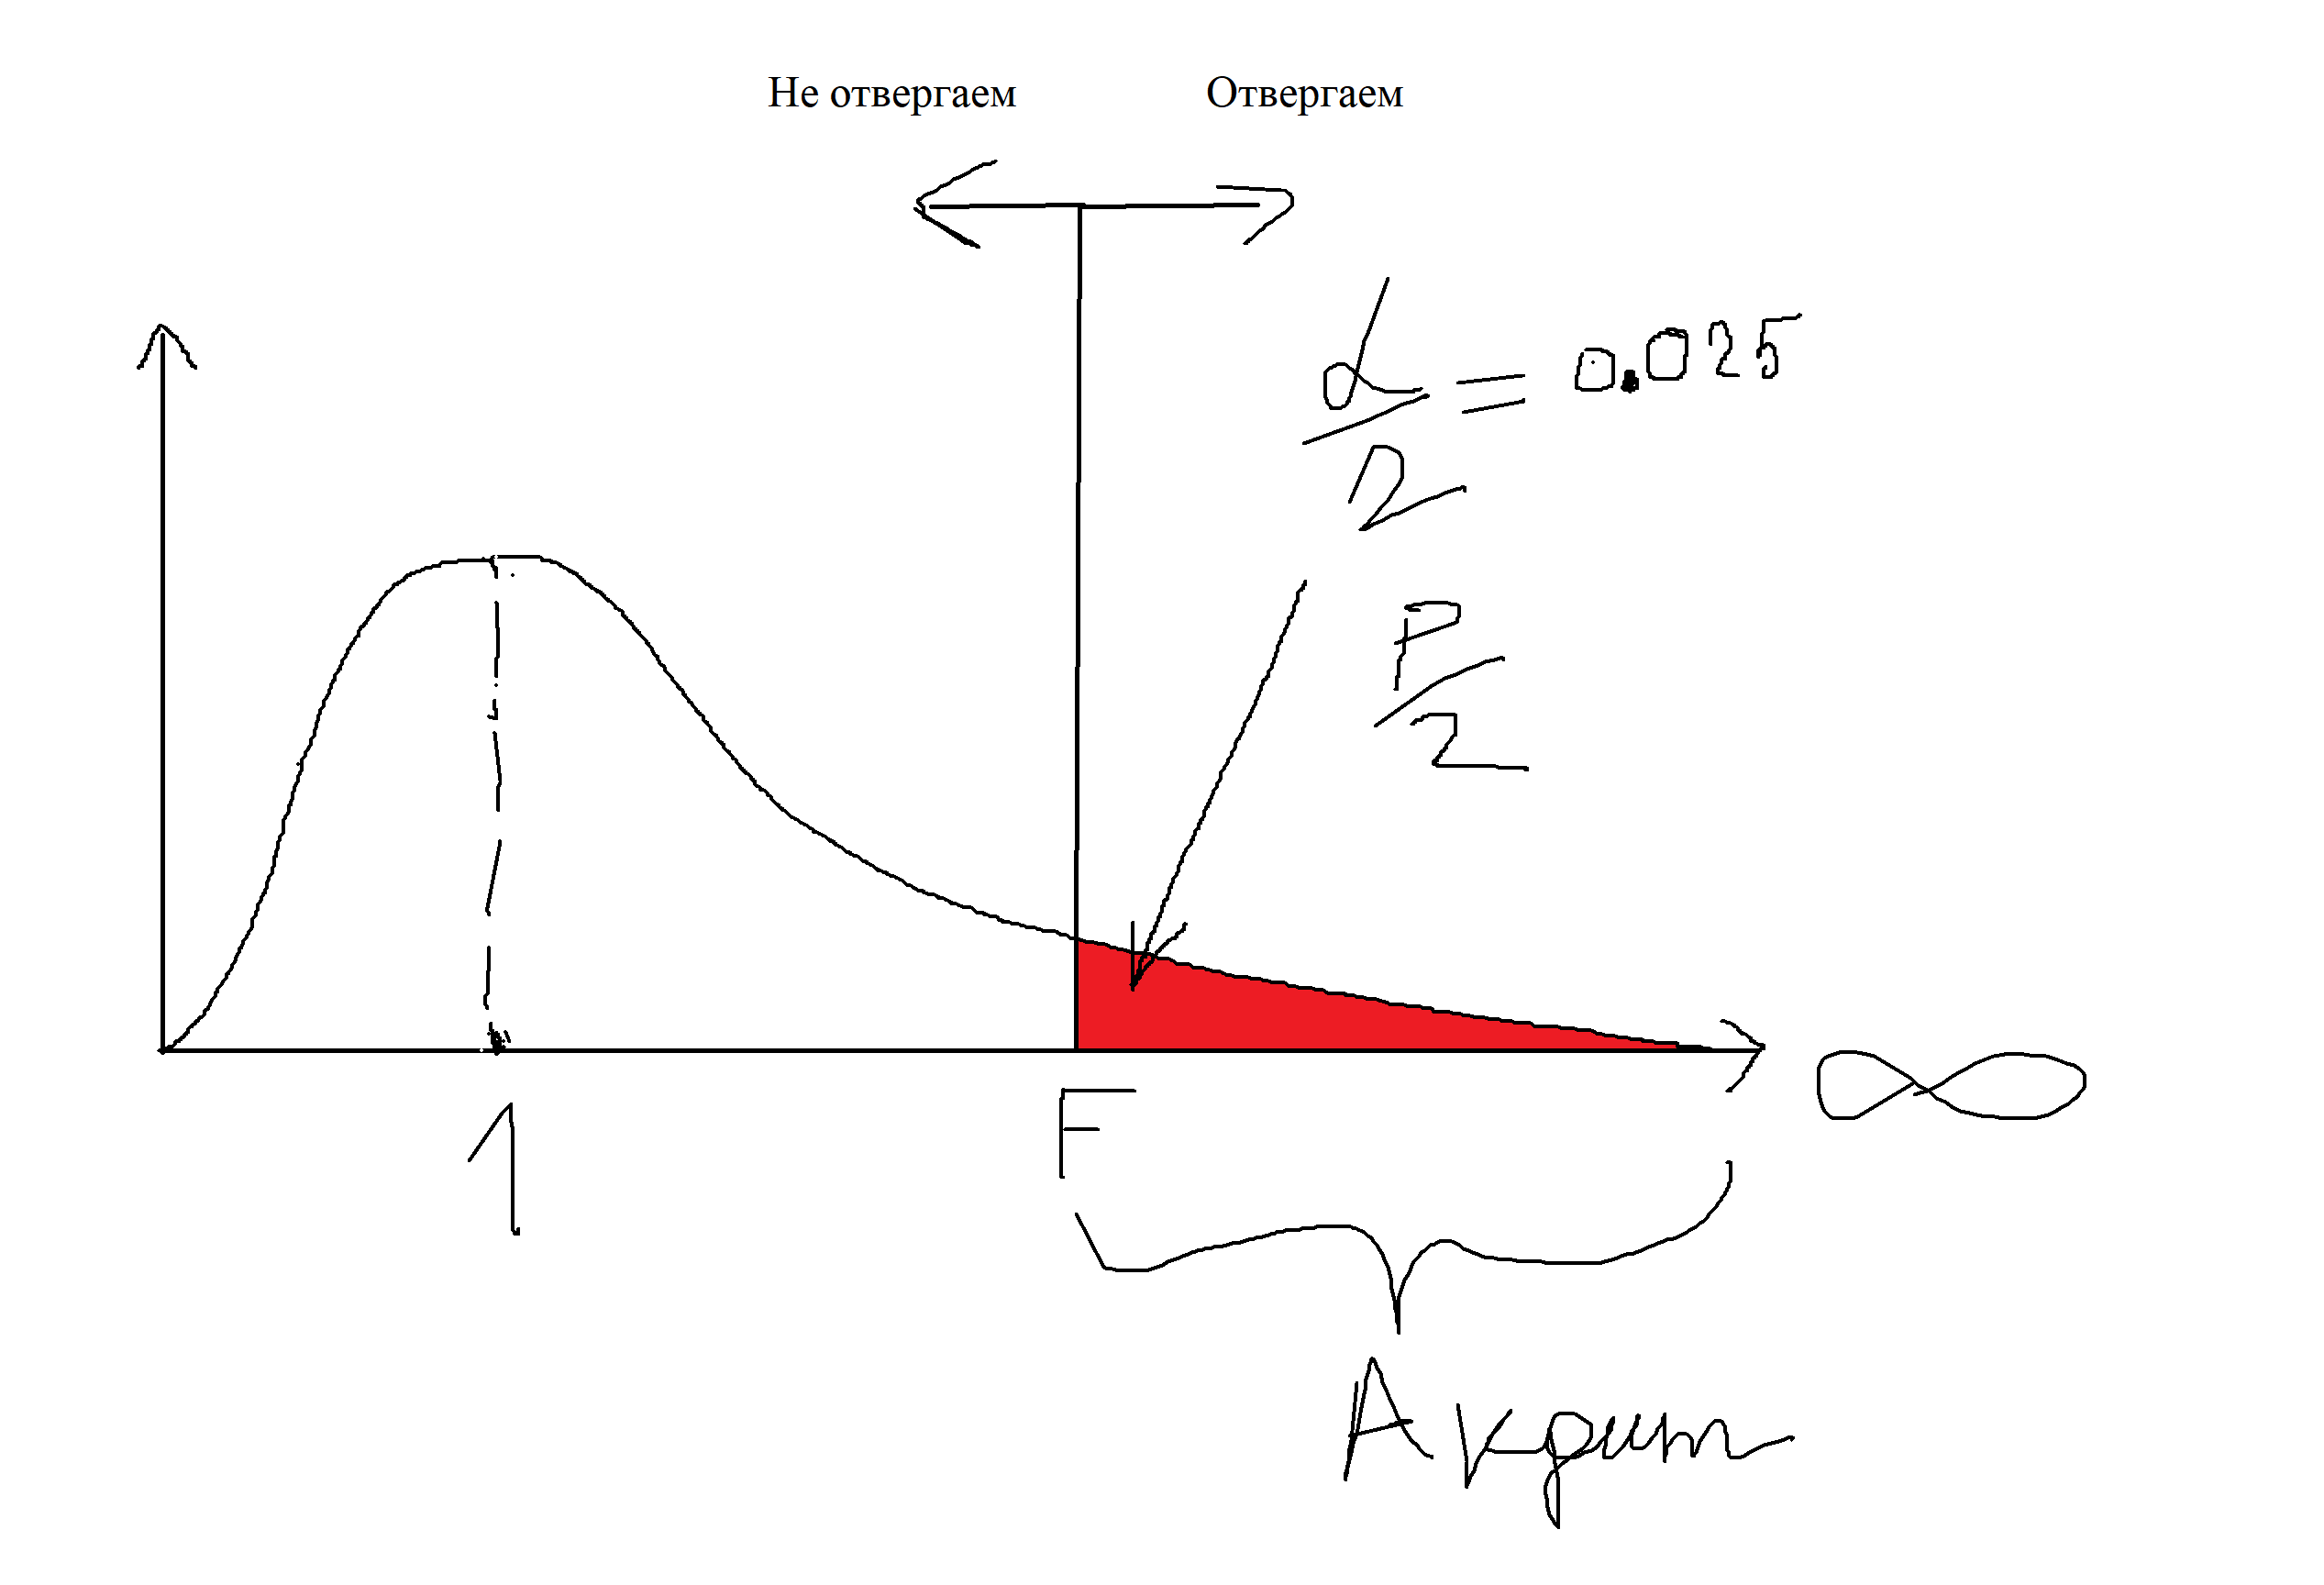
\includegraphics[width=0.8\linewidth]{Screenshot_2.png}
	\caption*{Рис. 0. Критическая область}
	\label{fig:mpr}
	
\end{figure*}
\setcounter{figure}{0}
\section*{Моделирование}
Для каждого распределения моделируются 10000 выборок размера 500 из соответствующего распределения, $\alpha = 0.05$, $\mathrm{H}_{0}: \quad \sigma_{1}^{2}=\sigma_{2}^{2}$, $\mathrm{H}_{1}: \quad \sigma_{1}^{2} \neq \sigma_{2}^{2}$.

\section*{Нормальное распределение}
Для начала два раза было сгенерировано 10 000 выборок размера 500 из нормального распределения $\mathcal{N}(0,\,1)$, т.е выборки соответствуют нулевой гипотезе о равенстве дисперсий. Далее был построен график распределения p-value (приложение 1, рисунок 1). Вероятность ошибки первого рода, указанная над графиком, равна выбранному уровню значимости, т.е. критерий является точным. 
\begin{figure}[hbt!]
	
	\centering
	
	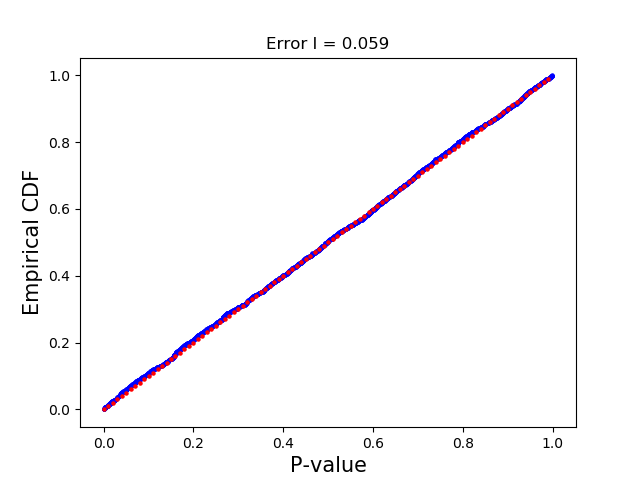
\includegraphics[width=0.8\linewidth]{Pvalue_normal_h0.png}
	\caption{Распределение p-value, нормальное распределение, $H_0$}
	\label{fig:mpr}
	
\end{figure}

Для альтернативной гипотезы о неравенстве дисперсий было сгенерировано 10 000 выборок размера 500 из $\mathcal{N}(0,\,1)$ и столько же из $\mathcal{N}(0,\,1.3)$. График распределения p-value представлен на рисунке 2 (код в приложении 2), ошибка второго рода практические равна 0, т.е. критерий обладает достаточной мощностью в случае нормального распределения.

\begin{figure}[hbt!]
	
	\centering
	
	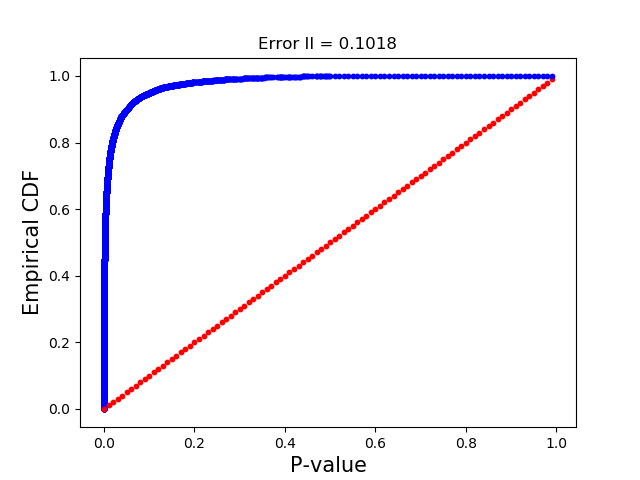
\includegraphics[width=0.8\linewidth]{Pvalue_normal_h1_alt.png}
	\caption{Распределение p-value, нормальное распределение, $H_1$}
	\label{fig:mpr}
	
\end{figure}
\subsection*{Логнормальное распределение}
Для построения функций распределения p-value два раза было сгенерировано 10 000 выборок размера 500 из логнормального распределения $Lognormal(\mu, \sigma^2)$ (несимметричное, коэф. эксцесса положительный) с параметрами $\mu = 0, \sigma^2 = 9/4$, то есть выборки соответствуют нулевой гипотезе о равенстве дисперсий. График распределения p-value для нулевой гипотезы представлен на рисунке 3, код программы в приложение 3.
\begin{figure}[hbt!]
	
	\centering
	
	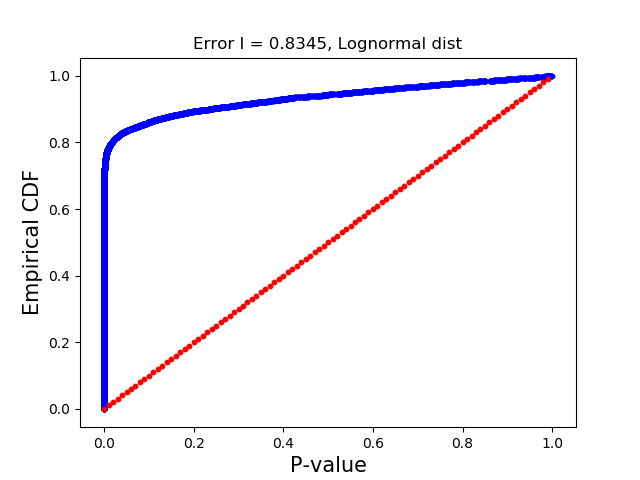
\includegraphics[width=0.8\linewidth]{Pvalue_longnormal_h0.png}
	\caption{Распределение p-value, логнормальное распределение, $H_0$}
	
	\label{fig:mpr}
	
\end{figure}

\subsection*{Распределение Лапласа}
 Для построения функций распределения p-value два раза было сгенерировано 10 000 выборок размера 500 из распределения Лапласа $Laplace(\mu, b)$ (симметричное, коэф. эксцесса положительный) с параметрами $\mu = 0, b = 2$, то есть выборки соответствуют нулевой гипотезе о равенстве дисперсий. График распределения p-value для нулевой гипотезы представлен на рисунке 4, код программы в приложение 4.
\begin{figure}[hbt!]
	\centering
	\includegraphics[width=0.8\linewidth]{Pvalue_laplace_h0.png}
	\caption{Распределение p-value, распределение Лапласа, $H_0$}
	\label{fig:mpr}
	
\end{figure}
\subsection*{Логистическое распределение}
 Для построения функций распределения p-value два раза было сгенерировано 10 000 выборок размера 500 из логистического распределения $Logistic(\mu, \beta)$ (симметричное, коэф. эксцесса положительный) с параметрами $\mu = 0, \beta = 2$, то есть выборки соответствуют нулевой гипотезе о равенстве дисперсий. График распределения p-value для нулевой гипотезы представлен на рисунке 5, код программы в приложение 5.
\begin{figure}[hbt!]
	\centering
	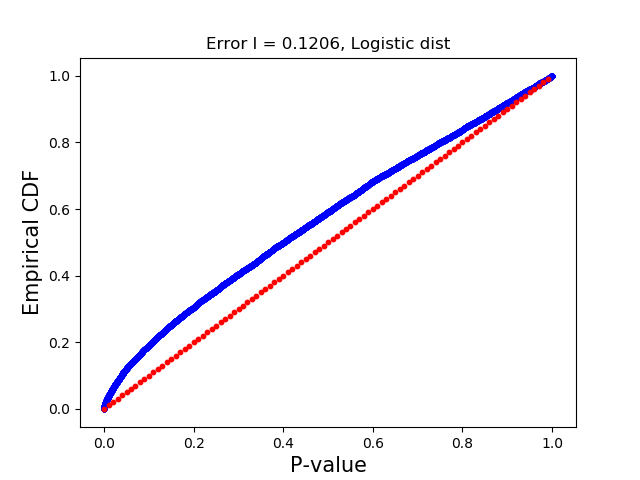
\includegraphics[width=0.8\linewidth]{Pvalue_logistic_h0.png}
	\caption{Распределение p-value, логистическое распределение, $H_0$}
	\label{fig:mpr}
\end{figure}

\newpage

\subsection*{Вывод}
Видно, что критерий в случае ненормальности распределения нельзя применять, он является радикальным. 

\subsection*{Проверка критерия на реальных данных}
В таблице на рисунке 6 представлены средние температуры за июль в городах Техаса и Калифорнии. Проверим данные на равенство дисперсий с помощью теста Фишера, $\alpha = 0.05$, $\mathrm{H}_{0}: \quad \sigma_{1}^{2}=\sigma_{2}^{2}$. Результат работы программы на языке Python (приложение 6) представлен на рисунке 7, p-value = 5.680033681176866e-06, что существенно меньше уровня значимости, следовательно гипотеза о равенстве дисперсий отвергается. 

\begin{figure}[h]
	\centering
	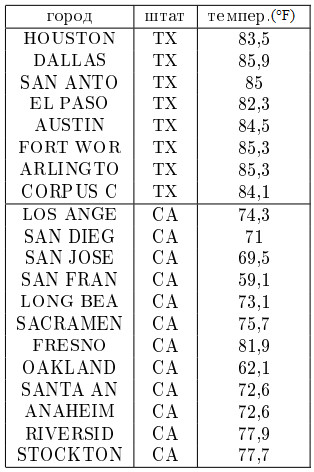
\includegraphics[width=0.4\linewidth]{table.png}
	\caption{Средне июльские температуры в Техасе и Калифорнии}
	\label{fig:mpr}
\end{figure}

\begin{figure}[h]
	\centering
	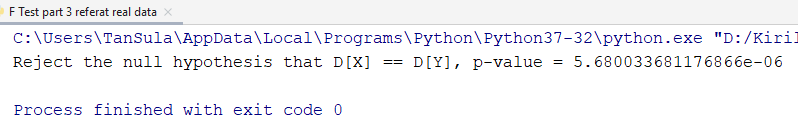
\includegraphics[width=0.8\linewidth]{Screenshot_1.png}
	\caption{Результат работы программы F-test}
	\label{fig:mpr}
\end{figure}

\clearpage
\section*{Приложение}

\subsection*{Приложение 1: Код программы на Python, Нормальное распределение, нулевая гипотеза, график p-value}
\begin{python}
from scipy.stats import norm
import scipy
import numpy as np
import matplotlib.pyplot as plt
import math

def ecdf(data):
    x = np.sort(data)
    n = x.size
    y = np.arange(1, n+1) / n
    return(x, y)


mean1, mean2 = 1, 1
var1, var2 = 1, 1
sigma1 = math.sqrt(var1)
sigma2 = math.sqrt(var2)
pval_size = 2000
sample_size = 200
error_1 = 0
alpha = 0.05
pval_data = [0 for i in range(pval_size)]
pval_data1 = [0 for i in range(pval_size)]
for i in range(pval_size):
    data1 = np.random.normal(mean1, sigma1, sample_size)
    data2 = np.random.normal(mean2, sigma2, sample_size)
    var1_ = data1.var()
    var2_ = data2.var()
    if var1_> var2_:
        F = var1_ / var2_
    else:
        F = var2_ / var1_
    df1, df2 = len(data1) - 1, len(data2) - 1
    p_value = (1-scipy.stats.f.cdf(F, df1, df2))*2
    pval_data[i] += p_value
    if p_value < alpha:
        error_1 += 1
x,y = ecdf(pval_data)
fig = plt.figure()
plt.scatter(x=x, y=y, s=5, c='b')
plt.title('Error I = %s' % (error_1/pval_size))
x_normal = [0.01*i for i in range(0, 100, 1)]
plt.scatter(x=x_normal, y=x_normal, color='red', s=5)
plt.xlabel('P-value', fontsize=15)
plt.ylabel('Empirical CDF', fontsize=15)
fig.savefig("Pvalue_normal_h0.png")
plt.show()
\end{python}

\subsection*{Приложение 2: Код программы на Python, Нормальное распределение, альтернативная гипотеза, график p-value}
\begin{python}
from scipy.stats import norm
import scipy
import numpy as np
import matplotlib.pyplot as plt
import math

def ecdf(data):
    x = np.sort(data)
    n = x.size
    y = np.arange(1, n+1) / n
    return x, y


mean1, mean2 = 1, 1
var1, var2 = 1, 1.7
sigma1 = math.sqrt(var1)
sigma2 = math.sqrt(var2)
pval_size = 2000
sample_size = 200
error_2 = 0
alpha = 0.05
pval_data = [0 for i in range(pval_size)]
pval_data1 = [0 for i in range(pval_size)]
for i in range(pval_size):
    data1 = np.random.normal(mean1, sigma1, sample_size)
    data2 = np.random.normal(mean2, sigma2, sample_size)
    var1_ = data1.var()
    var2_ = data2.var()

    if var1_> var2_:
        F = var1_ / var2_
    else:
        F = var2_ / var1_

    df1, df2 = len(data1) - 1, len(data2) - 1
    p_value = 2*(1-scipy.stats.f.cdf(F, df1, df2))
    pval_data[i] += p_value

    if p_value > alpha:
        error_2 += 1

x,y = ecdf(pval_data)
fig = plt.figure()
plt.scatter(x=x, y=y)
plt.title('Error II = %s' % (error_2 / pval_size))
x_normal = [0.01*i for i in range(0, 100, 1)]
plt.scatter(x=x_normal, y=x_normal, color='red', s=10)
plt.xlabel('P-value', fontsize=15)
plt.ylabel('Empirical CDF', fontsize=15)
fig.savefig("Pvalue_normal_h1.png")
plt.show()
\end{python}

\subsection*{Приложение 3: Код программы на Python, Логонормальное распределение, нулевая гипотеза, график p-value}
\begin{python}
from scipy.stats import lognorm
import scipy
import math
import numpy as np
import matplotlib.pyplot as plt


def ecdf(data):
    x = np.sort(data)
    n = x.size
    y = np.arange(1, n+1) / n
    return(x, y)


mean = 0
var1, var2 = 9/4, 9/4
sigma1 = math.sqrt(var1)
sigma2 = math.sqrt(var2)
pval_size = 2000
sample_size = 20000
alpha = 0.05
error_1 = 0
pval_data = [0 for i in range(pval_size)]

for i in range(pval_size):

    data1 = np.random.lognormal(mean, sigma1, sample_size)
    data2 = np.random.lognormal(mean, sigma2, sample_size)
    var1_, var2_ = data1.var(), data2.var()

    if var1_ > var2_:
        F = var1_ / var2_
    else:
        F = var2_ / var1_

    df1, df2 = len(data1) - 1, len(data2) - 1
    p_value = 2*(1-scipy.stats.f.cdf(F, df1, df2))
    pval_data[i] += p_value

    if p_value < alpha:
        error_1 += 1

x,y = ecdf(pval_data)
fig = plt.figure()
plt.scatter(x=x, y=y, s=10, color='blue')
x_normal = [0.01*i for i in range(0, 100, 1)]
plt.scatter(x=x_normal, y=x_normal, color='red', s=10, label='-1')
plt.title('Error I = %s, Lognormal dist' % (error_1/pval_size))
plt.xlabel('P-value', fontsize=15)
plt.ylabel('Empirical CDF', fontsize=15)
fig.savefig("Pvalue_longnormal_h0.png")
plt.show()
\end{python}

\subsection*{Приложение 4: Код программы на Python, распределение Лапласа, нулевая гипотеза, график p-value}
\begin{python}
from scipy.stats import lognorm, laplace
import scipy
import numpy as np
import matplotlib.pyplot as plt


def ecdf(data):
    x = np.sort(data)
    n = x.size
    y = np.arange(1, n+1) / n
    return(x, y)


from scipy.stats import lognorm
import scipy
import math
import numpy as np
import matplotlib.pyplot as plt


def ecdf(data):
    x = np.sort(data)
    n = x.size
    y = np.arange(1, n+1) / n
    return(x, y)


mean = 0
var1, var2 = 2, 2
scale1, scale2 = var1/2, var2/2
sigma2 = math.sqrt(var2)
pval_size = 2000
sample_size = 20000
alpha = 0.05
error_1 = 0
pval_data = [0 for i in range(pval_size)]

for i in range(pval_size):

    data1 = np.random.laplace(mean, scale=scale1, size=sample_size)
    data2 = np.random.laplace(mean, scale=scale2, size=sample_size)
    var1_, var2_ = data1.var(), data2.var()

    if var1_ > var2_:
        F = var1_ / var2_
    else:
        F = var2_ / var1_
    df1, df2 = len(data1) - 1, len(data2) - 1
    p_value = 2*(1-scipy.stats.f.cdf(F, df1, df2))
    pval_data[i] += p_value

    if p_value < alpha:
        error_1 += 1

x,y = ecdf(pval_data)
fig = plt.figure()
plt.scatter(x=x, y=y, s=10, c='b')
x_normal = [0.01*i for i in range(0, 100, 1)]
plt.scatter(x=x_normal, y=x_normal, color='red', s=10, label='-1')
plt.title('Error I = %s, Laplace dist'% (error_1/pval_size))
plt.xlabel('P-value', fontsize=15)
plt.ylabel('Empirical CDF', fontsize=15)
fig.savefig("Pvalue_laplace_h0.png")
plt.show()
\end{python}

\subsection*{Приложение 5: Код программы на Python, Логистическое распределение, нулевая гипотеза, график p-value}
\begin{python}
from scipy.stats import norm
import scipy
import numpy as np
import matplotlib.pyplot as plt
from math import *


def ecdf(data):
    x = np.sort(data)
    n = x.size
    y = np.arange(1, n+1) / n
    return x, y


scale1, scale2 = 2, 2
loc = 5
var1 = (scale1**2)*(pi**2)/3
var2 = (scale2**2)*(pi**2)/3
pval_size = 10000
sample_size = 500
error_1 = 0
alpha = 0.05
pval_data = [0 for i in range(pval_size)]
pval_data1 = [0 for i in range(pval_size)]
for i in range(pval_size):
    data1 = np.random.logistic(loc=loc, scale=scale1, size=sample_size)
    data2 = np.random.logistic(loc=loc, scale=scale2, size=sample_size)
    var1_ = data1.var()
    var2_ = data2.var()

    if var1_> var2_:
        F = var1_ / var2_
    else:
        F = var2_ / var1_
    df1, df2 = len(data1) - 1, len(data2) - 1
    p_value = (1-scipy.stats.f.cdf(F, df1, df2))*2
    pval_data[i] += p_value

    if p_value < alpha:
        error_1 += 1
x,y = ecdf(pval_data)
x_normal = [0.01*i for i in range(0, 100, 1)]
fig = plt.figure()
ax = fig.add_subplot(111)
ax.scatter(x=x, y=y, color='blue', s=10, label='1')
ax.scatter(x=x_normal, y=x_normal, color='red', s=10, label='-1')
plt.title('Error I = %s, Logistic dist' % (error_1/pval_size))
plt.xlabel('P-value', fontsize=15)
plt.ylabel('Empirical CDF', fontsize=15)
fig.savefig("Pvalue_logistic_h0.png")
plt.show()
\end{python}

\subsection*{Приложение 5: Код программы на Python, F-test для реальных данных}
\begin{python}
import scipy
import math
import random
import numpy as np
import matplotlib.pyplot as plt
from scipy.stats import norm


n = 200
alpha = 0.05
data1 = [83.5, 85.9, 85.3, 82.3, 84.5, 85.3, 85.3, 84.1]
data2 = [74.3, 71, 69.5, 59.1, 73.1, 75.7, 81.9, 62.1, 72.6, 72.6, 77.9, 77.7]
n1, n2 = len(data1), len(data2)
mean1_, mean2_ = sum(data1) / n1, sum(data2) / n2
var1_ = sum((x - mean1_)**2 for x in data1) / (n1 - 1)
var2_ = sum((x - mean2_)**2 for x in data2) / (n2 - 1)
if var1_> var2_:
    F = var1_ / var2_
else:
    F = var2_ / var1_
df1, df2 = len(data1) - 1, len(data2) - 1
p_value = 2*(1-scipy.stats.f.cdf(F, df1, df2))
if p_value < alpha:
    print('Reject the null hypothesis that D[X] == D[Y], p-value = %s' % p_value)
else:
    print('Can not reject the null hypothesis that D[X] == D[Y], p-value = %s' % p_value)
\end{python}
\end{document}
